\documentclass[12pt,a4paper]{article}
\usepackage{cmap} % Makes the PDF copiable. See http://tex.stackexchange.com/a/64198/25761
\usepackage[T1]{fontenc}
\usepackage[brazil]{babel}
\usepackage[utf8]{inputenc}
\usepackage{amsmath}
\usepackage{amsfonts}
\usepackage{amssymb}
\usepackage{amsthm}
\usepackage{textcomp} % \degree
\usepackage{gensymb} % \degree
\usepackage[usenames,svgnames,dvipsnames]{xcolor}
\usepackage{hyperref}
\usepackage{multicol}
\usepackage{graphicx}
\usepackage[margin=2cm]{geometry}

\hypersetup{
    colorlinks = true,
    allcolors = {blue}
}

% TODO: Consider using exsheets
% http://linorg.usp.br/CTAN/macros/latex/contrib/exsheets/exsheets_en.pdf
%
% http://ctan.org/tex-archive/macros/latex/contrib/exercise/
% Options: answerdelayed,lastexercise,noanswer
\usepackage[answerdelayed,lastexercise]{exercise}

\addto\captionsbrazil{%
\def\listexercisename{Lista de exerc\'icios}%
\def\ExerciseName{Exerc\'icio}%
\def\AnswerName{Solu\c{c}\~ao do exerc\'icio}%
\def\ExerciseListName{Ex.}%
\def\AnswerListName{Solu\c{c}\~ao}%
\def\ExePartName{Parte}%
\def\ArticleOf{de\ }%
}

\renewcommand{\ExerciseHeaderTitle}{(\ExerciseTitle)\ }
\renewcommand{\ExerciseListHeader}{%\ExerciseHeaderDifficulty%
\textbf{%\ExerciseListName\
\ExerciseHeaderNB.\ %
%\ --- \
\ExerciseHeaderTitle}%
%\ExerciseHeaderOrigin
\ignorespaces}
\renewcommand{\AnswerListHeader}{\textbf{\ExerciseHeaderNB.\ (\AnswerListName)\ }}

\newcommand*\sen{\operatorname{sen}}
\newcommand*\dom[1]{\operatorname{Dom}\left(#1\right)}
\newcommand*\R{\mathbb{R}}

\renewcommand{\theenumi}{\alph{enumi}}
\renewcommand\labelenumi{(\theenumi) }
\renewcommand{\theenumii}{\roman{enumii}}

\newcommand*\tipo{Prova III (parte 2)}
\newcommand*\turma{TADS121-01U}
\newcommand*\disciplina{CDI0001}
\newcommand*\eu{Helder G. G. de Lima}
\newcommand*\data{20/11/2017}

\author{\eu}
\title{\tipo - \disciplina}
\date{\data}

\begin{document}
\thispagestyle{empty}
\newgeometry{margin=2cm,bottom=0.5cm}
\begin{center}

\includegraphics[width=9.0cm]{marca} \\
\textbf{\tipo\ (\disciplina / \turma)} \\
Prof. \eu\footnote{
Este é um material de acesso livre distribuído sob os termos da licença \href{https://creativecommons.org/licenses/by-sa/4.0/deed.pt_BR}{Creative Commons Atribuição-CompartilhaIgual 4.0 Internacional}}
\end{center}

\noindent Nome do(a) aluno(a): \underline{\hspace{9,7cm}} Data: \underline{\data}

\begin{center}\fbox{
\begin{minipage}{14cm}

{\footnotesize
\begin{itemize}
\renewcommand{\theenumi}{\Roman{enumi}}
\item Identifique-se em todas as folhas.
\item Mantenha o celular e os demais equipamentos eletrônicos desligados durante a prova.
\item Justifique cada resposta com cálculos ou argumentos baseados na teoria estudada.
\item Escolha e responda apenas 4 das 5 questões, totalizando 8,0 pontos.
\end{itemize}
}

\end{minipage}
}
\end{center}

\begin{ExerciseList}
\Exercise[title={2,0}] Calcule os limites a seguir utilizando, se necessário, as regras de L'Hôpital:
\begin{enumerate}
\item $\displaystyle\lim_{x \to 1} \frac{x^3 - 3 x^2 - 3 x + 5}{\sen(\pi x) \cdot \cos(\pi x)}$
\item $\displaystyle\lim_{x \to -\infty} x^2 e^{3x}$
\end{enumerate}
\Answer
\begin{enumerate}
\item Como o numerador e o denominador tendem a zero, pode-se usar a regra de L'Hôpital para obter:
\begin{align*}
\lim_{x \to 1} \frac{x^3 - 3 x^2 - 3 x + 5}
               {\sen(\pi x) \cdot \cos(\pi x)}
& =\lim_{x \to 1} \frac{3x^2 - 6x - 3}
                {\cos(\pi x) \cdot \pi \cdot \cos(\pi x) + \sen(\pi x)\cdot (-\sen(\pi x) \cdot \pi) }\\
& =\frac{3 - 6 - 3}
   {-1 \cdot \pi \cdot (-1) + 0 \cdot (-0 \cdot \pi) }
= -\frac{6}{\pi}
\end{align*}
\item Como um dos fatores tende a infinito e o outro tende a zero, podemos reescrever o limite de modo a aplicar a regra de L'Hôpital:
\begin{align*}
\lim_{x \to -\infty} x^2 e^{3x}
= \lim_{x \to -\infty} \frac{ x^2 }{ e^{-3x} }
= \lim_{x \to -\infty} \frac{ 2x }{ -3e^{-3x} }
= \lim_{x \to -\infty} \frac{ 2 }{ 9e^{-3x} }
= 0
\end{align*}
\end{enumerate}

\Exercise[title={2,0}] Encontre o ponto pertencente à reta $r: 2x + y = 10$ que está mais próximo da origem. Justifique (usando cálculo diferencial) por que o ponto encontrado é, de fato, o mais próximo.

{\footnotesize
(Lembre-se que a distância entre os pontos $A=(x_0,y_0)$ e $B=(x_1,y_1)$ é $\operatorname{d}(A,B) = \sqrt{(x_1-x_0)^2 + (y_1-y_0)^2}$)
}
\Answer Considerando $A = (x, y) \in r$ tem-se $y=10-2x$ e se $B = (0,0)$ então
\[
d(A,B) = d(x)
= \sqrt{x^2 + (10-2x)^2}
= \sqrt{x^2 + (100 -40x + 4x^2)}
= \sqrt{5x^2-40x + 100}
\]
Assim,
\[
d^\prime(x)
= \frac{ 10x - 40 }{2\sqrt{5x^2-40x + 100} }
= \frac{ 5x - 20 }{\sqrt{5x^2-40x + 100} }
\]

Assim, $d^\prime(x) = 0$ se, e somente se, $5x-20 = 0$, isto é, $x=\frac{20}{5} = 4$. Para $x>4$ tem-se $5x-20 > 0$ e portanto $d^\prime(x) > 0$ e $d$ é crescente. Por outro lado, se $x<4$ então $5x-20 < 0$ e consequentemente $d^\prime(x) < 0$ e $d$ é decrescente. Logo $x=4$ é um ponto de mínimo da função distância, ou seja, $A = (4, 10-2\cdot 4) = (4, 2)$ é o ponto da reta que está mais próximo da origem.

\Exercise[title={2,0}] Suponha que $f:\R \to \R$ é uma função derivável com as seguintes propriedades:
\begin{multicols}{3}
\begin{itemize}
\item $f^\prime(1) = 0$
\item $f^\prime(x) > 0$ se $x < 1$
\item $f^\prime(x) < 0$ se $x > 1$
\item $f^{\prime\prime}(2) = 0$
\item $f^{\prime\prime}(x) < 0$ se $x < 2$
\item $f^{\prime\prime}(x) > 0$ se $x > 2$
\item $\displaystyle\lim_{x \to -\infty} f(x) = -\infty$
\item $\displaystyle\lim_{x \to +\infty} f(x) = 0$
\end{itemize}
\end{multicols}
É possível garantir que $f$ possui algum ponto de máximo local? E de mínimo local? E de inflexão? Explique suas respostas e exemplifique como poderia ser o gráfico de $f$ se ela satisfizesse todas as condições dadas. Indique claramente no gráfico todos os pontos relevantes.
\Answer Com base nas informações dadas sobre $f^\prime$ e $f^{\prime\prime}$, pode-se dizer que:
\begin{itemize}
\item A função $f$ é crescente em $(-\infty, 1)$ e decrescente em $(1, +\infty)$, ou seja, $P = (1, f(1))$ é um ponto de máximo local de $f$.
\item Como $f$ é derivável, para que houvesse um ponto de mínimo em $x = a$, a função $f^\prime$ precisaria ser negativa para $x < a$ e positiva para $x>a$. Mas isso não ocorre em nenhum ponto $a \in \R$, então $f$ não possui ponto de mínimo.
\item Como $f^{\prime\prime}(x) < 0$ para $x \in (-\infty, 2)$ e $f^{\prime\prime} (x)> 0$ em $x \in (2, +\infty)$, conclui-se que há uma mudança de concavidade no ponto $Q = (2, f(2))$, ou seja, $Q$ é um ponto de inflexão de $f$.
\end{itemize}
Com base nas informações anteriores, o gráfico poderia ser o seguinte:
\begin{center}
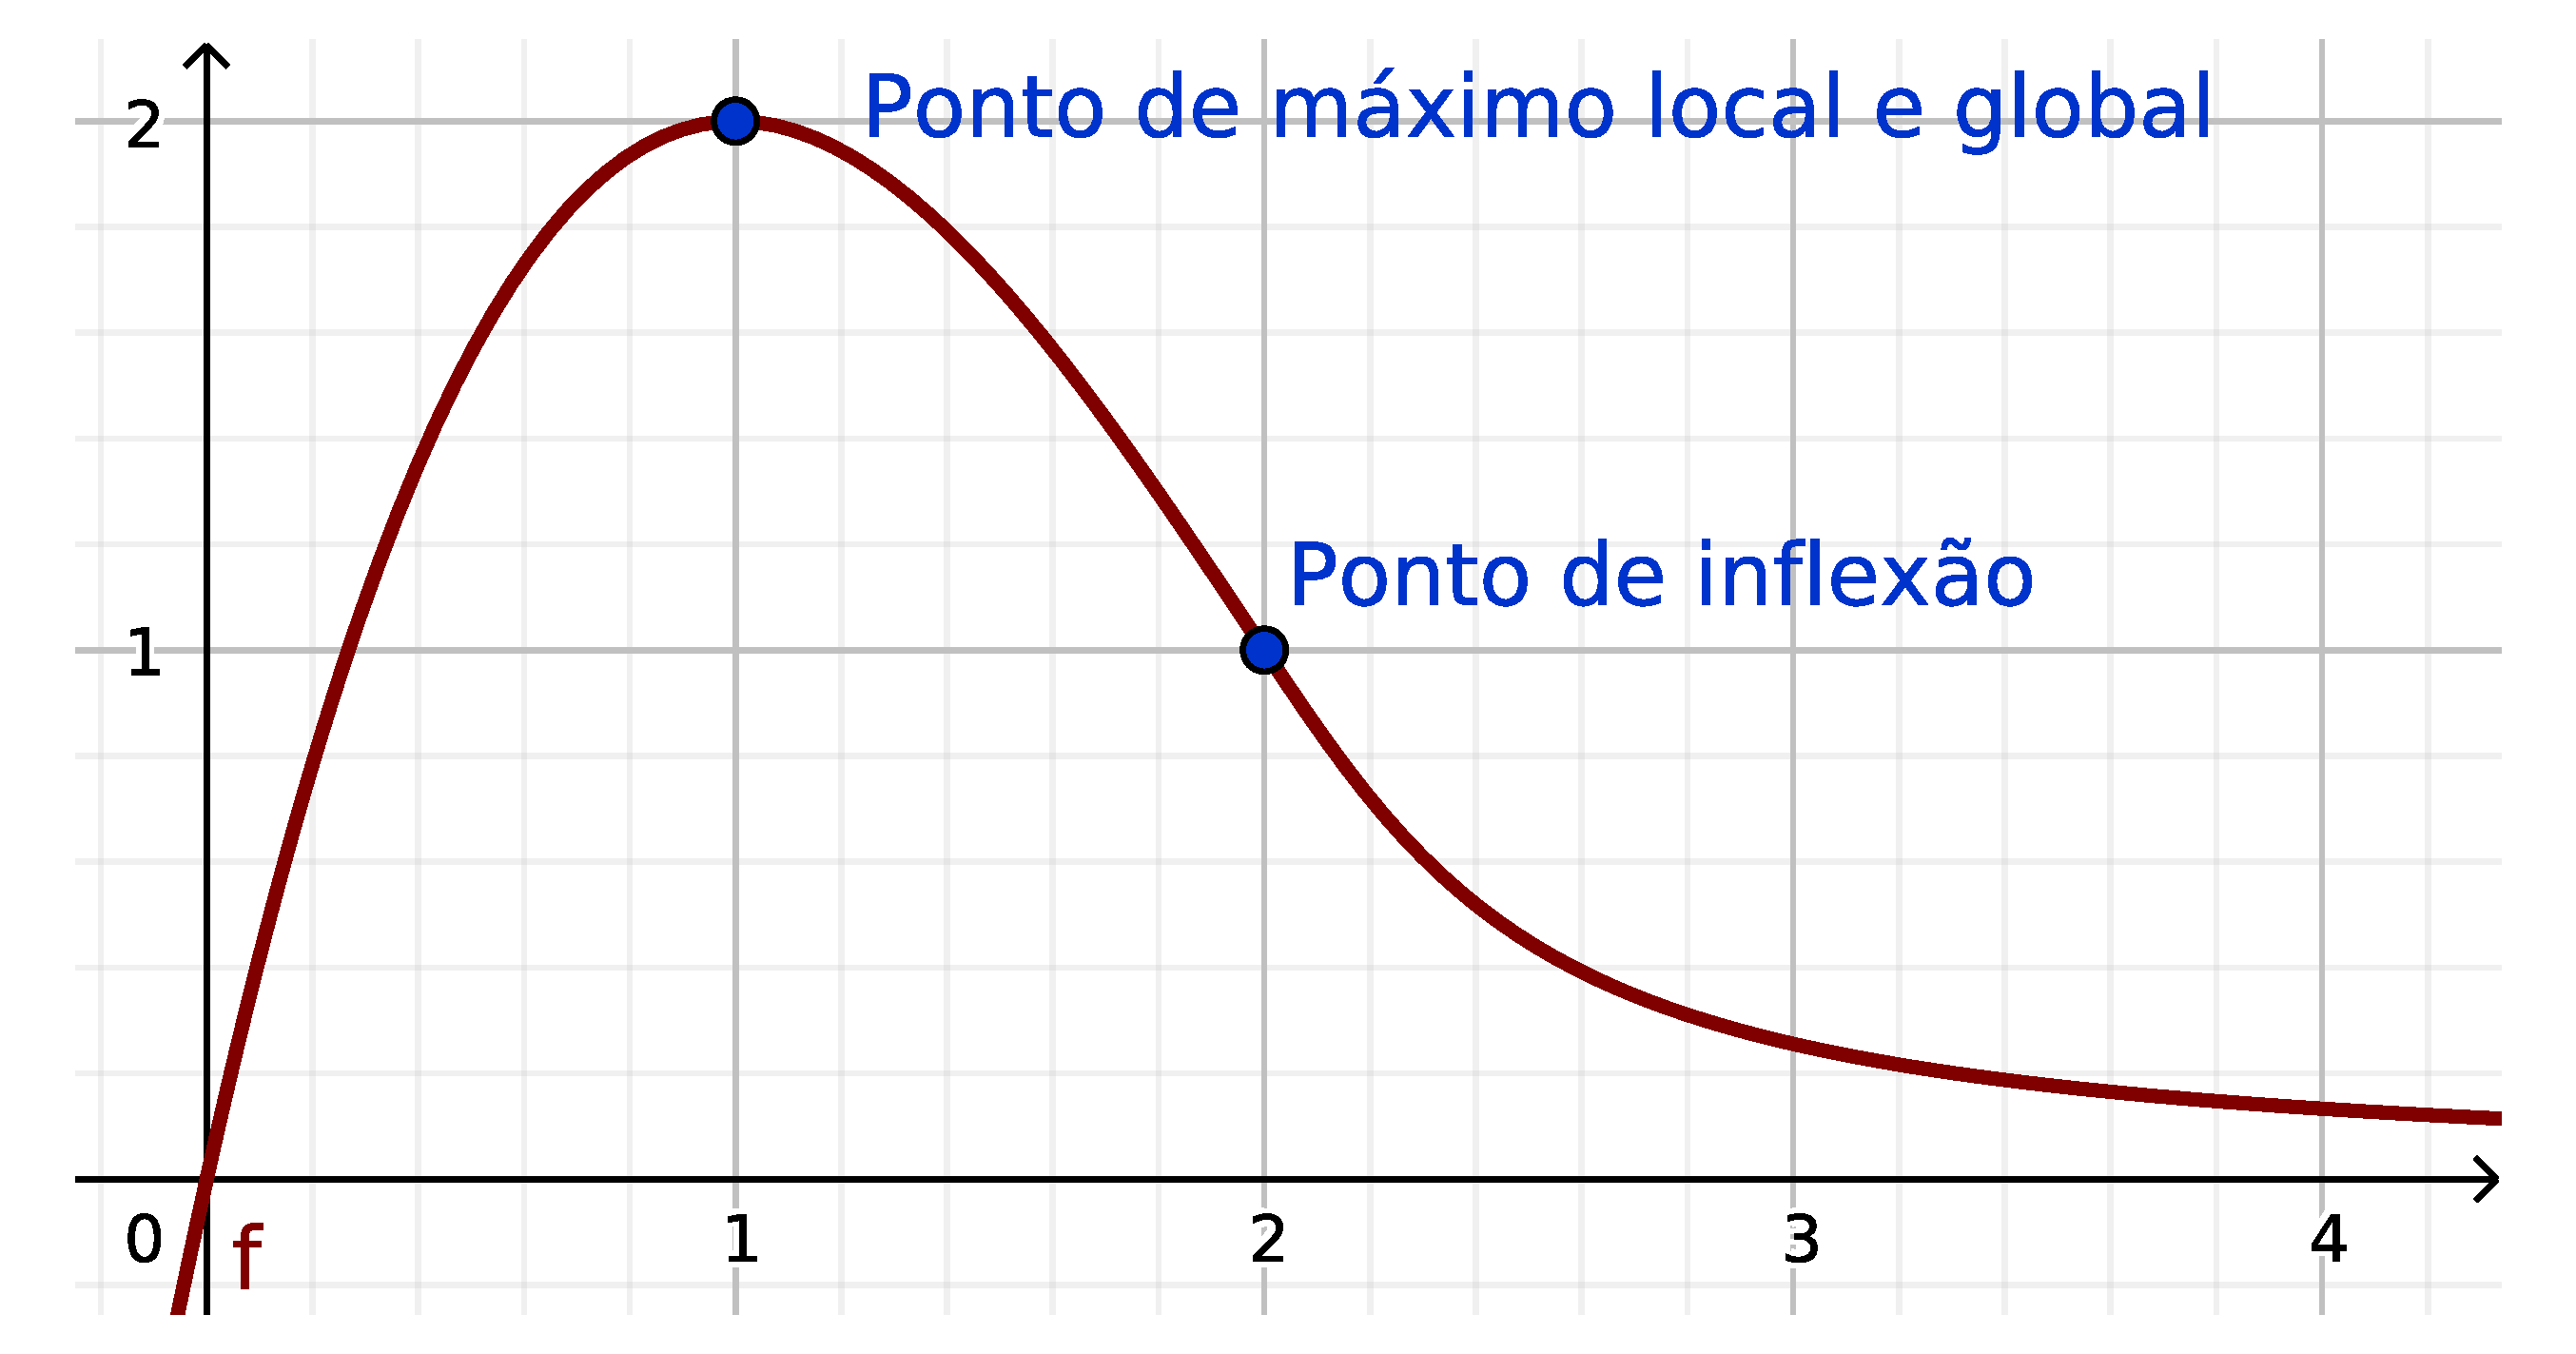
\includegraphics[width=11.0cm]{img/prova-3-tads-graph}
\end{center}

\Exercise[title={2,0}] Obtenha todas as assíntotas, de todos os tipos, da função $g(x) = \dfrac{3x^2 + \ln(x)}{x}$.
\Answer
Primeiramente, note que $\dom{g} = (0, +\infty)$ e que em $x_0 = 0$ tem-se
\[
  \lim_{x \to x_0+} g(x)
= \lim_{x \to 0+} \dfrac{3x^2 + \ln(x)}{x}
= \lim_{x \to 0+} 3x + \dfrac{1}{x} \cdot \ln(x) = -\infty.
\]
Logo, $x=0$ é uma assíntota vertical de $g$. Além disso, em $+\infty$, pode-se aplicar a regra de L'Hôpital para obter:
\[
  \lim_{x \to +\infty} g(x)
= \lim_{x \to +\infty} \dfrac{3x^2 + \ln(x)}{x}
= \lim_{x \to +\infty} \dfrac{6x + \frac{1}{x}}{1}
= +\infty
\]
Isso implica que não há uma assíntota horizontal. Por outro lado, como
\[
a = \lim_{x \to +\infty} \frac{ g(x) }{ x }
= \lim_{x \to +\infty} \dfrac{3x^2 + \ln(x)}{x^2}
= \lim_{x \to +\infty} \dfrac{6x + \frac{1}{x}}{2x}
= \lim_{x \to +\infty} \dfrac{6 -\frac{1}{x^2}}{2}
= 3
\]
e
\[
b = \lim_{x \to +\infty} g(x) - ax
= \lim_{x \to +\infty} \dfrac{3x^2 + \ln(x)}{x}-3x
= \lim_{x \to +\infty} \dfrac{3x^2 + \ln(x) -3x^2}{x}
= \lim_{x \to +\infty} \dfrac{\ln(x)}{x}
= \lim_{x \to +\infty} \dfrac{\frac{1}{x}}{1}
= 0
\]
conclui-se que a reta $y = 3x$ é uma assíntota oblíqua de $g$.

\Exercise[title={2,0}] Em qual/quais ponto(s) $x \in \R$ a reta tangente ao gráfico de $y = x^3(2x^2-15x+30)$ tem a sua maior inclinação? Justifique sua resposta.
\Answer Como a inclinação da reta tangente ao gráfico de certa função é dada pela derivada da função no ponto correspondente, a questão consiste em identificar o(s) máximo(s) da função $h(x) = y^\prime(x)$. Pelas regras de derivação, tem-se:
\begin{align*}
h(x) = y^\prime
& = ( 2x^5-15x^4+30x^3 )^\prime
  = 10x^4-60x^3+90x^2
\end{align*}
e como $\lim_{x \to +\infty} 10x^4-60x^3+90x^2 = +\infty$, as retas tangentes ao gráfico tendem a ficar mais inclinadas conforme $x$ aumenta, ou seja, não há um valor máximo (global).
\end{ExerciseList}

\newpage
\restoregeometry
\section*{Respostas}
\shipoutAnswer
\end{document}
